\documentclass[a4paper,12pt]{article}
\usepackage[utf8]{inputenc}
\usepackage{todonotes}
\usepackage[russian]{babel}
\usepackage{graphicx}
\usepackage{amsmath, amssymb}
\usepackage{hyperref}
\usepackage{float}
\usepackage{listings}
\usepackage{caption}
\usepackage{geometry}
\usepackage{xcolor}
\usepackage{todo}
\geometry{left=2cm,right=2cm,top=2cm,bottom=2cm}
\hypersetup{pdfborder=0 0 0}
\pagestyle{fancy}
\headsep=8mm
\footskip=20mm
\hypersetup{pdfstartview=FitH, linkcolor=linkcolor, urlcolor=urlcolor, colorlinks=true}

\definecolor{strings}{rgb}{0,0.6,0}
\definecolor{comments}{rgb}{0,0.3,0}
\definecolor{numbers}{rgb}{0.5,0.5,0.5}
\definecolor{keywords}{rgb}{0.09,0.61,0.95}
\definecolor{background}{rgb}{0.97,0.97,0.97}

\lstdefinestyle{codestyle}{
    backgroundcolor=\color{background},
    commentstyle=\color{comments},
    keywordstyle=\color{keywords},
    stringstyle=\color{strings},
    numberstyle=\tiny\color{numbers},
    basicstyle=\ttfamily\scriptsize,
    breakatwhitespace=false,
    breaklines=true,
    captionpos=b,
    inputencoding=utf8,
    keepspaces=false,
    numbers=left,
    numbersep=5pt,
    showspaces=false,
    showstringspaces=false,
    showtabs=false,
    tabsize=2,
    extendedchars=true
}

\lstset{style=codestyle}

\begin{document}

% Титульный лист
\begin{titlepage}
    \centering
    {\large Федеральное государственное автономное образовательное учреждение\par}
    {\large высшего образования\par}
    {\bfseries САНКТ-ПЕТЕРБУРГСКИЙ НАЦИОНАЛЬНЫЙ ИССЛЕДОВАТЕЛЬСКИЙ УНИВЕРСИТЕТ ИТМО\par}
    {\bfseries Факультет систем управления и робототехники\par}
    \vfill
    {\Large \bfseries Лабораторная работа №2\par}
    {\Large \bfseries Геометрические преобразования изображений\par}
    \vfill
    
    \begin{flushright}
        Студенты: & Бахтаиров Р.А.,\\ Сайфуллин Д.Р. \\
        Поток: & Тех.Зр R23 1.1 \\
        Преподаватель: & Шаветов С.В.
    \end{flushright}
    \vfill
    Санкт-Петербург, 2025 г.
\end{titlepage}

% Оглавление
\tableofcontents
\newpage

% Введение
\section{Цель работы}
Целью этой работы будет изучение методов геометрических преобразований изображений. Когда эти методы можно применить, а когда и обратить. 
\section{Изображение, которое будем использовать для проверки функций}
\begin{figure}[H]
    \centering 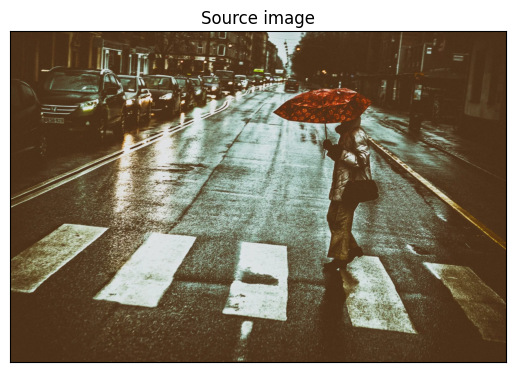
\includegraphics[width=0.7\textwidth]{my_images/1.png}
    \caption{Изначальное изображение}
\end{figure}

% Основной код
\section{Изначальный код работы}
Весь код работы будет находится в прикреплённом файле. Далее в работе будут разбираться методы, которые мы применили в этом коде, но не он сам.
\\
\url{https://drive.google.com/file/d/19y2GYcEUAg_iHPJK4L0hfDuE9uBK_dD8/view?usp=sharing}
\section{Простейщие геометрические преобразования}
В этом разделе описаны методы преобразования изображений, используемые в лабораторной работе.
\begin{enumerate}
    \item предисловие и однородные системы координат
    \item Линейные преобразования
    \begin{itemize}
        \item смещение
        \item переворот
        \item изменение масштаба/растяжение
        \item поворот
        \item аффинные преобразования
        \item кусочные
    \end{itemize}
    \item Нелинейные преобразования
      \begin{itemize}
        \item перспективное
        \item полиномиальная
        \item синусоидальное искажение
    \end{itemize}
\end{enumerate}
\
Подробно разберём каждое из них 
\subsection{предисловие и однородные системы координат}
Изображения это плоские объекты, каждый из которых можно описать пикселем с его положением и интенсивностью. В декартовой системе координат каждому пикселю соответсвуют набор значений (x,y). За счёт этого и свойств линейности довольно большое количество преобразований изображений можно применить просто сменив базис(т.е умножив на матрицу).
\
Тем не менее есть ограничения из-за которых не все операции можно представить в виде матриц. Для разрешения этой проблемы вводять однородные координаты $(x,y,\omega )$. $\omega$ - Это скаляр масштабирования, который изначально равен 1:
$$
	\begin{bmatrix} x' \\ y' \\ w \end{bmatrix} = w
	\begin{bmatrix} x \\ y \\ 1 \end{bmatrix}
	\Leftrightarrow
	\begin{bmatrix} x' & y' & w \end{bmatrix} =
	\begin{bmatrix} x & y & 1 \end{bmatrix}w
$$
За счёт добавления этой координаты мы можем применять сдвиг с помощью матрицы 3*3
$$
	\Leftrightarrow
	\begin{bmatrix} x' \\ y' \\ 1 \end{bmatrix} =
	\begin{bmatrix}
		A & B & C
		\\ D & E & F
		\\ 0 & 0 & 1
	\end{bmatrix} \cdot
	\begin{bmatrix} x \\ y \\ 1 \end{bmatrix}
$$
$$
	\begin{cases}
		x'=Ax+By+C,
		\\ y'=Dx+Ey+F
	\end{cases}
$$
\
*OpenCV сохраняет такое преобразование как матрицу 2*2 и вектор смещения.
\subsection{Линейные преобразования}
Линейные преобразования сохраняют бесконечно малые фигуры и угол между кривыми и их точками пересечения.
\subsubsection{Смещение изображения}
данное преобразвание смещает все пиксели изображения на один вектор
Матрица такого преобразования выглядит таким образом(при условии, если векторы 1*3)
$$
	T =
	\begin{bmatrix}
		1 & 0 & 0
		\\ 0 & 1 & 0
		\\ C & F & 1
	\end{bmatrix}
$$
Применять в OpenCV мы будет её в таком виде:
$$
	T =
	\begin{bmatrix}
		1 & 0 & C
		\\ 0 & 1 & F
	\end{bmatrix},
$$
Т.е у транспонированной матрицы обрезаем последнию строчку, не несущую информацию об преобразовании. 
Для правильного отображения этого преобразования после его применения необходимо изменять разрешение изображения. 
Ниже представлены примеры этого преобразования
\begin{figure}[H]
    \centering 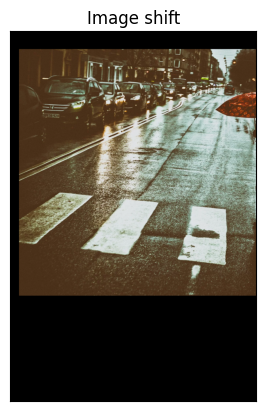
\includegraphics[width=0.7\textwidth]{my_images/3.png}
    \caption{смещение, если забыть об изменении разрешения изображения}
\end{figure}
\begin{figure}[H]
    \centering 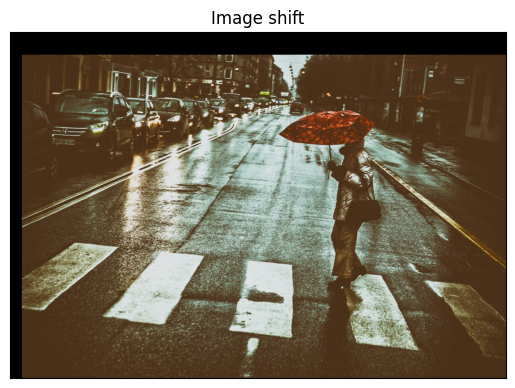
\includegraphics[width=0.7\textwidth]{my_images/5.png}
    \caption{Смещение с положительными коэффициентами}
\end{figure}
\begin{figure}[H]
    \centering 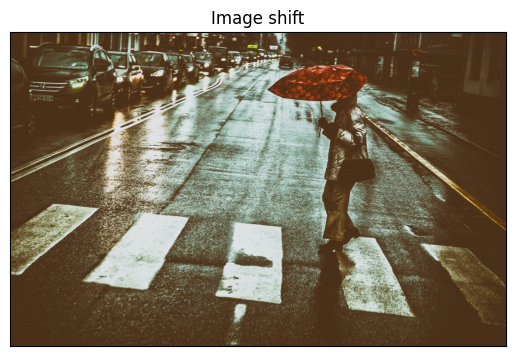
\includegraphics[width=0.7\textwidth]{my_images/7.png}
    \caption{Отрицательное смещение(изображение обрезалось)}
\end{figure}
\subsubsection{Переворот изображения}
Для переворота изображения относительно одной из осей достаточно умножить соответсвующий базисный вектор на -1. Тем не менее, так как мы имеем ограниченную и сторого положительную область отображения, то одновременно с этим необходимо также сделать смещение. 
В таком случае матрица отражения относительно оси x:
$$
	T =
	\begin{bmatrix}
		1 & 0 & 0
		\\ 0 & -1 & I.rows - 1
	\end{bmatrix}
$$
а вот, к примеру, относительно y 
$$
	T =
	\begin{bmatrix}
		-1 & 0 & I.columns - 1
		\\ 0 & 1 & 0
	\end{bmatrix}
$$
\begin{figure}[H]
    \centering 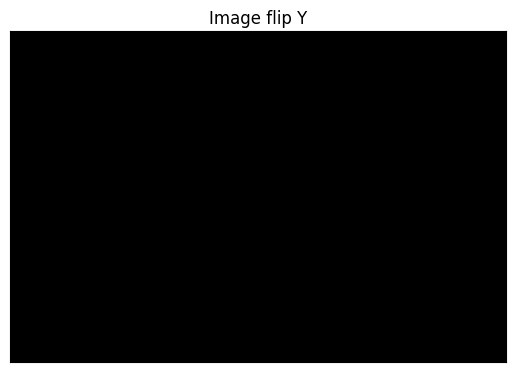
\includegraphics[width=0.7\textwidth]{my_images/9.png}
    \caption{Если забыть о смещении}
\end{figure}
\begin{figure}[H]
    \centering 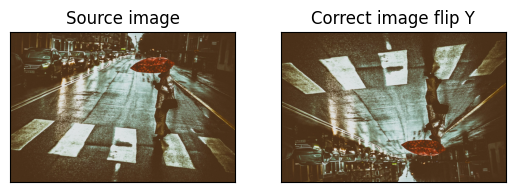
\includegraphics[width=0.7\textwidth]{my_images/10.png}
    \caption{Переворот оси y}
\end{figure}
\begin{figure}[H]
    \centering 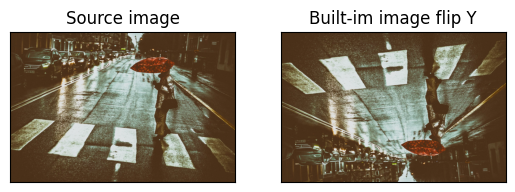
\includegraphics[width=0.7\textwidth]{my_images/11.png}
    \caption{Переворот оси y от OpenCV}
\end{figure}
\begin{figure}[H]
    \centering 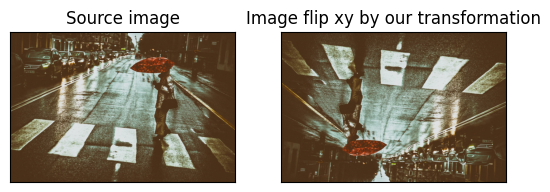
\includegraphics[width=0.7\textwidth]{my_images/12.png}
    \caption{Переворот сразу по 2 осям}
\end{figure}
Наше отображение полностью совпало с тем, что выдаёт встроенная функция в OpenCV
\subsubsection{Растяжение изображения}
Данное отображение довольно очевидным образом представляется в виде матрицы
$$
	\begin{cases}
		x'={\alpha}x, \alpha > 0 \\
		y'={\beta}y, \beta > 0
	\end{cases}
	\Rightarrow
	T=
	\begin{bmatrix}
		\alpha & 0 & 0
		\\ 0 & \beta & 0
		\\ 0 & 0 & 1
	\end{bmatrix}
$$
И случай для 
$$
	T =
	\begin{bmatrix}
		\alpha & 0 & 0
		\\ 0 & \beta & 0
	\end{bmatrix},
$$
Подводным камнем данного отображения является необходимость граммотного изменения разрешения изображения. Также стоит понимать, что в этом отображение уже могут возникать потери. Именно из-за них, к примеру, наше отображение с помощью матрицы попиксельно не совпадает с тем, что полученно с помощью встроенной в openCV функции, хотя по сути выглядят они одинаково(openCV после масштабирования всегда применяют интеполяцию пустых пикселей)
\begin{figure}[H]
    \centering 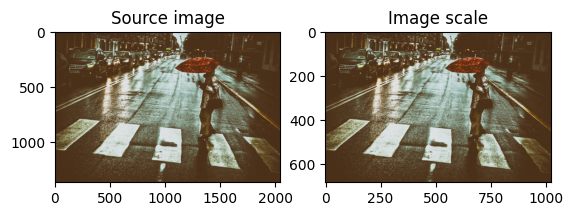
\includegraphics[width=0.7\textwidth]{my_images/14.png}
    \caption{Уменьшили разрешение}
\end{figure}
\begin{figure}[H]
    \centering 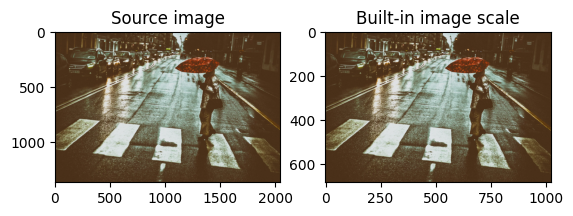
\includegraphics[width=0.7\textwidth]{my_images/15.png}
    \caption{Уменьшили разрешение с помощью средств OpenCV}
\end{figure}
\begin{figure}[H]
    \centering 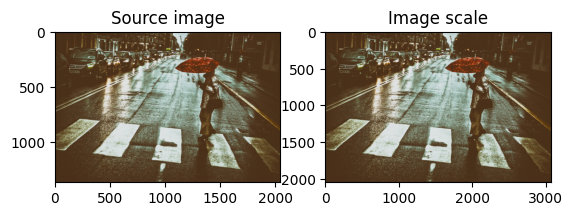
\includegraphics[width=0.7\textwidth]{my_images/16.png}
    \caption{Увеличили разрешение}
\end{figure}
\begin{figure}[H]
    \centering 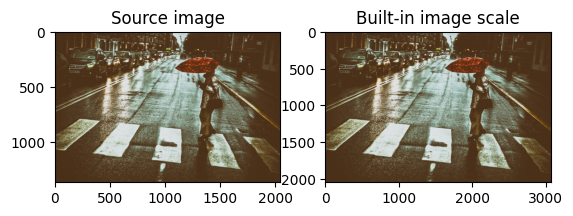
\includegraphics[width=0.7\textwidth]{my_images/17.png}
    \caption{Увеличили разрешение с помощь OpenCV}
\end{figure}
\subsubsection{поворот}
Матрица данной трансформации
$$
	\begin{cases}
		x'=x \cos \varphi - y \sin \varphi \\
		y'=x \sin \varphi + y \cos \varphi
	\end{cases}
	\Rightarrow
	T=
	\begin{bmatrix}
		{\cos \varphi} & {-\sin \varphi} & 0
		\\ {\sin \varphi} & {\cos \varphi} & 0
		\\ 0 & 0 & 1
	\end{bmatrix}
$$
Классическая матрица поворота по часовой стрелке. Важно понимать, что поворот происходит вокруг начала координат отсчёта пиксей(в openCV он в верхнем левом углу). Если же поворот необходимо выполнить относительно другой оси, необходиом последовательно применить череду нескольких линейных преобразований
$$T = T_{shiftback} \times T_{rotate} \times T_{shift}$$
Т.е смещение к точке, поворот, возврат к изначальному положению.
\begin{figure}[H]
    \centering 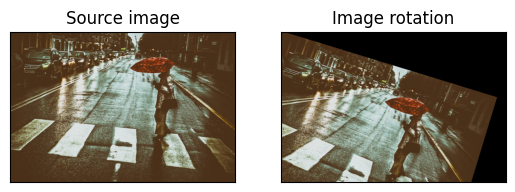
\includegraphics[width=0.7\textwidth]{my_images/18.png}
    \caption{поворот на небольшой угол}
\end{figure}
\begin{figure}[H]
    \centering 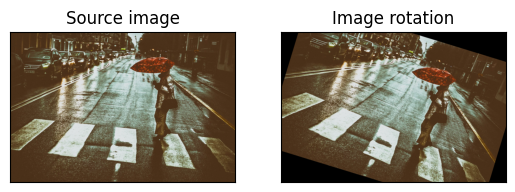
\includegraphics[width=0.7\textwidth]{my_images/19.png}
    \caption{поворот на небольшой угол с осью в центре изображения}
\end{figure}
\begin{figure}[H]
    \centering 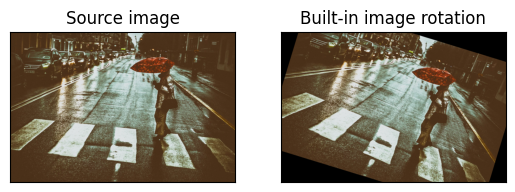
\includegraphics[width=0.7\textwidth]{my_images/20.png}
    \caption{поворот на небольшой угол с помощью OpenCV}
\end{figure}
\begin{figure}[H]
    \centering 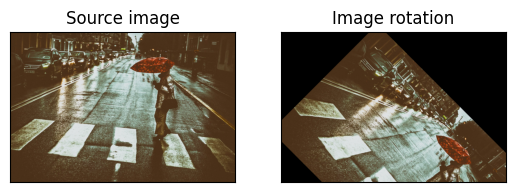
\includegraphics[width=0.7\textwidth]{my_images/21.png}
    \caption{поворот на угол 45 $\degree$}
\end{figure}
\begin{figure}[H]
    \centering 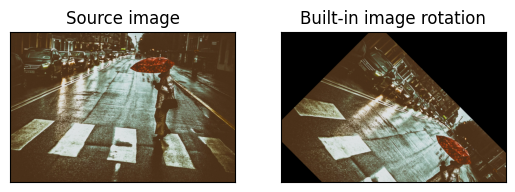
\includegraphics[width=0.7\textwidth]{my_images/22.png}
    \caption{поворот на угол 45 $\degree$ c помощь OpenCV}
\end{figure}
Преобразование через матрицу опять попиксельно не совпало со встроенным. Из за ошибок округления возникли пустые пиксели, который встроенный метод заполним с помощью интерполяции(в отличии от нашего)
\subsubsection{Произвольное аффинное преобразование}
Для нахождения произвольного аффинного преобразования нам достаточно определить 3 пары точек $P_{src} = \lbrace(x_1, y_1), (x_2, y_2), (x_3, y_3)\rbrace$ $P_{dst} = \lbrace(x'_1, y'_1), (x'_2, y'_2), (x'_3, y'_3)\rbrace$. 
И просто решается система:
$$
	\begin{cases}
    x'_1 = x_1 \cdot A + y_1 \cdot B + C \\
    y'_1 = x_1 \cdot D + y_1 \cdot E + F \\
    x'_2 = x_2 \cdot A + y_2 \cdot B + C \\
    y'_2 = x_2 \cdot D + y_2 \cdot E + F \\
    x'_3 = x_3 \cdot A + y_3 \cdot B + C \\
    y'_3 = x_3 \cdot D + y_3 \cdot E + F
  \end{cases}
$$
С помощью которой мы находим необходимые для матрицы коэффициенты. Как можно понять, если мы возьмем точки, лежащие на одной прямой, то система станет вырожденной, так что лучше этого избежать. 
Матрицу мы находим с помощью метода.  \texttt{cv.getAffineTransform()}
Довольно любопытно, что если поменять соответсвующие точки местами(x' и x и т.д), то мы получим обратную матрицу для данного преобразования( но не всегда получится избежать потерь данных)
\begin{figure}[H]
    \centering 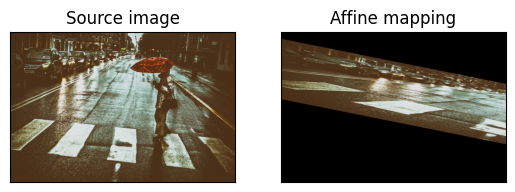
\includegraphics[width=0.7\textwidth]{my_images/23.png}
    \caption{Аффинное преобразование}
\end{figure}
\begin{figure}[H]
    \centering 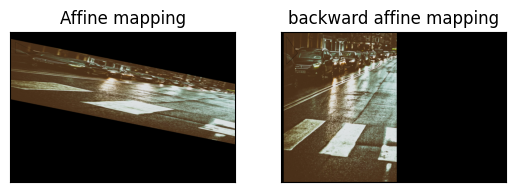
\includegraphics[width=0.7\textwidth]{my_images/24.png}
    \caption{обратное аффиному преобразование}
\end{figure}
Как мы видим, полностью изображения востановить не получилось.
\subsubsection{Скос}
Матрица скоса орта, отвечающего за координату x
$$
	\begin{cases}
		x'=x+sy, \\
		y'=y,
	\end{cases}
	\Rightarrow
	T=
	\begin{bmatrix}
		1 & 0 & 0
		\\ s & 1 & 0
		\\ 0 & 0 & 1
	\end{bmatrix}
$$
Очевидно, коэффициент s можно переставить и к орту y.
\begin{figure}[H]
    \centering 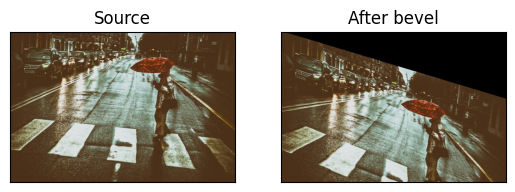
\includegraphics[width=0.7\textwidth]{my_images/25.png}
    \caption{Скос}
\end{figure}
Как можно заметить, название "скос" полностью подходит для этого преобразования
\subsubsection{ кусочные}
Кусочные преобразования отличаются от предыдущих только тем, что они применяются только к определённой части изображения. Вот некоторые примеры:
\begin{figure}[H]
    \centering 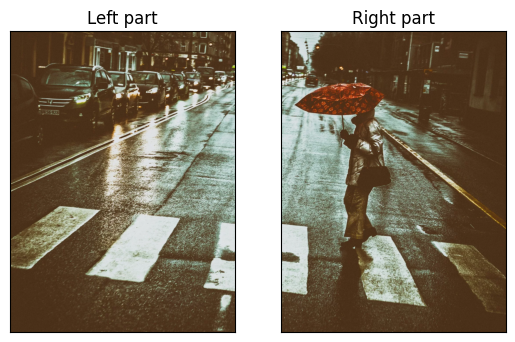
\includegraphics[width=0.7\textwidth]{my_images/26.png}
    \caption{Изображение, поделённое на части}
\end{figure}
\begin{figure}[H]
    \centering 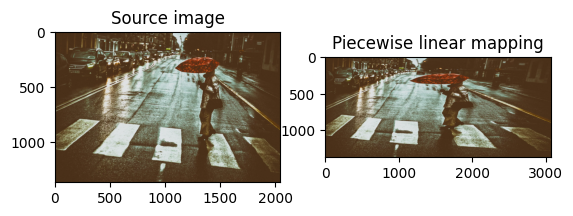
\includegraphics[width=0.7\textwidth]{my_images/27.png}
    \caption{Растянули левую часть в 2 раза}
\end{figure}
\begin{figure}[H]
    \centering 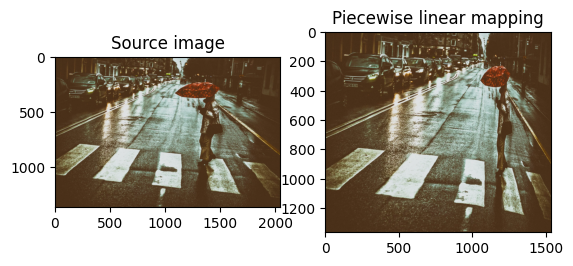
\includegraphics[width=0.7\textwidth]{my_images/30.png}
    \caption{Сжали правую часть в два раза}
\end{figure}
\subsection{Нелинейные преобразования}
В нелинейных преобразования прямые линии до преборазования становятся кривыми. Рассмотрим некоторые из нелинейных преобразований. 
\subsubsection{Перспективное}
Как мы помним перспективное отображение по своей сути является отображением из трёмерного изображения в двухмерное. В этом плане оно чем-то напоминает проекционное, только вот в перспективном размер изображния обратнопропорционально зависит от расстояния до "камеры". Именно это "обратнопропорциональность" и делает перспективные преобразование нелинейным. 
В данном случае нам очень пригодится то, что мы используем однородные  координаты. В матрице преобразования будем использовать свободную нижнию строку. А "под копотом" будем после применения линейного преобразования делить на координату $\omega$, тем самым создавая нелинейность. 
$$
	\begin{cases}
		x'=\dfrac{Ax+By+C}{Gx+Hy+I}, \\
		y'=\dfrac{Dx+Ey+F}{Gx+Hy+I},
	\end{cases}
	\Rightarrow
	T=
	\begin{bmatrix}
		A & B & C
		\\ D & E & F
		\\ G & H & 1
	\end{bmatrix}
$$
OpenCV использует для этого преобразования \texttt{cv.warpPerspective}
и \texttt{cv.getPerspectiveTransform()}. В случае  \texttt{cv.getPerspectiveTransform()} мы не используем матрицу, а выбираем 4 точки до преобразования и после. Как можно понять, данная функция решит систему сверху и построит по ней матрицу.
Мы также можем менять местами точки в парах, чтобы создавать обратное к перспективному отображение. 
\begin{figure}[H]
    \centering 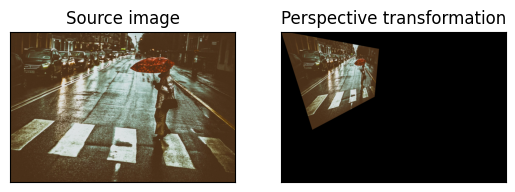
\includegraphics[width=0.7\textwidth]{my_images/31.png}
    \caption{Перспективное преобразование}
\end{figure}
\begin{figure}[H]
    \centering 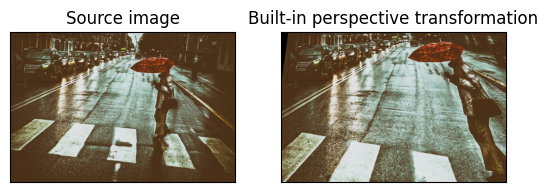
\includegraphics[width=0.7\textwidth]{my_images/32.png}
    \caption{Другое перспективное преобразование}
\end{figure}
\begin{figure}[H]
    \centering 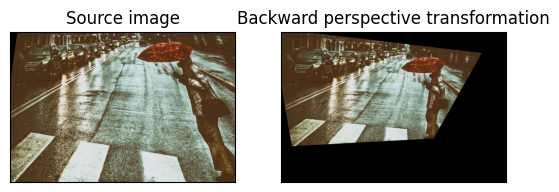
\includegraphics[width=0.7\textwidth]{my_images/33.png}
    \caption{Обратное преспективному преобразование}
\end{figure}
Как можно видеть, потерь изобежать не получилось, но вот сама выделенная область выглядит довольно интересно 
\subsubsection{Полиномиальное преобразование}
Довольно прямолинейное отображение
$$
	\begin{cases}
		x'=a_1+a_2x+a_3y+a_4x^2+a_5xy+a_6y^2 \\
		y'=b_1+b_2x+b_3y+b_4x^2+b_5xy+b_6y^2
	\end{cases}
$$
Воспользовавшись довольно прямолинейное заменой получаем преобразования, выгядящие так:
\begin{figure}[H]
    \centering 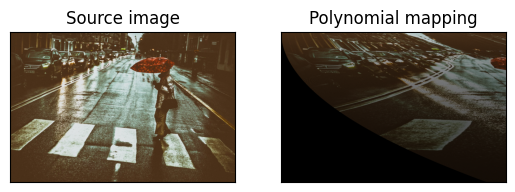
\includegraphics[width=0.7\textwidth]{my_images/34.png}
    \caption{Полиномиальное преобразование}
\end{figure}
\begin{figure}[H]
    \centering 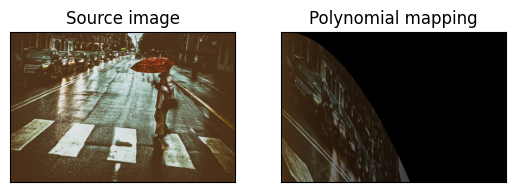
\includegraphics[width=0.7\textwidth]{my_images/35.png}
    \caption{Ещё одно полиномиальное преобразование}
\end{figure}
видно, как последнее из них идет слева направо. Это связано с тем, что вдоль оси x у нас просто линейная часть с коэффициентом 1.
\subsubsection{Синусоидальное искажение}
Вдоль одной оси каждому пикселю мы прибавляем значения синуса, зависящае от от координаты вдоль этой самой оси. К примеру при x=1 мы ко всем точкам (1,y) прибавим sin(1). Такое преобразование можно делать в доль любой оси.
\begin{figure}[H]
    \centering 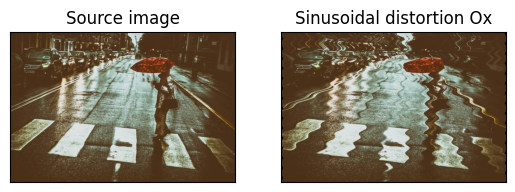
\includegraphics[width=0.7\textwidth]{my_images/36.png}
    \caption{Синусоидальное искажение вдоль оси y(но искажается координата x)}
\end{figure}
\begin{figure}[H]
    \centering 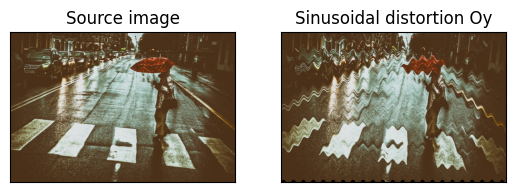
\includegraphics[width=0.7\textwidth]{my_images/37.png}
    \caption{Синусоидальное искажение вдоль оси x(но искажается координата y)}
\end{figure}
Выгляти довольно любопытно. Также стоит обратить внимание, что если сделать амплитуду синуса достаточной большой, то тогда возникнуть заметные проблемы.
\section{Исправление искажения}
В данном разделе мы будем исправлять искажения изображения, которые обычно возникают в том или ином виде при использовании камеры из-за оптических свойств линз. 
Такие искажения обычно можно представить в виде функции
$$
	\vec{R}=b_0\vec{r}+F_3r^2\vec{r}+F_5r^4\vec{r}+\dots
$$
центром отчёта является главная оптическая ось, т.е центр фотографии. Как нам известно, не зависимо от вида линзы, лучи, проходящие через центр, не искажаются. 
В данном разделе мы будем работать со следующими видами искажений
\begin{enumerate}
    \item barrel(бочкообразное)
    \item Pincushion(подушкообразное)
\end{enumerate}
Оба из них являются нелинейными. Их отличительной черной является то, что для их использования мы переходим к полярной системе координат, а само искажение мы делаем зависимым только от одной переменной(r-удалённость от центра).
\subsection{бочкообразное искажение}
Для построения этого искажения мы используем полином 5-ого порядка. 
Важной частью в коде является переход к системе координат от центра изображения + переход к полярным координатам. Далее мы применяем наше искажения, а после возращаемся к прямоугольной системе координат. 
\begin{figure}[H]
    \centering 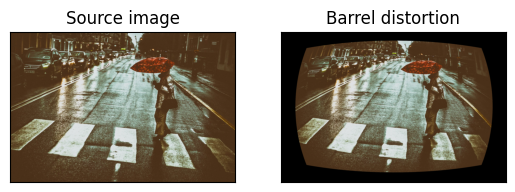
\includegraphics[width=0.7\textwidth]{my_images/38.png}
    \caption{Бочкообразное искажение}
\end{figure}
Довольно интересным методом мы востанавливаем искаженное изображение. В коде мы в неявном виде пользуемся матрицей Вандермонда для того, чтобы найти полином, который бы обращал это искажения. В каком-то смылсе мы этот нелинейный объект пытаемся вычислить с помощью линейных методов. Как можно видеть, эти методы довольно эффективны, но стоит понимать, что ошибки будут возникать при увеленичении значений коэффициентов. 
\begin{figure}[H]
    \centering 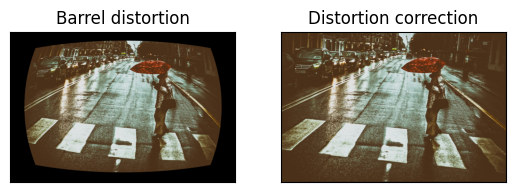
\includegraphics[width=0.7\textwidth]{my_images/39.png}
    \caption{Востановление искажения}
\end{figure}
\begin{figure}[H]
    \centering 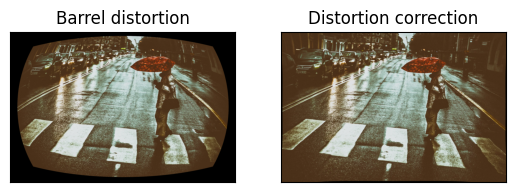
\includegraphics[width=0.7\textwidth]{my_images/40.png}
    \caption{Ещё один пример}
\end{figure}
Если обратить внимания на края, то можно увидеть что наша "линейная" апроксимация испытывает некоторые сложности на самых краях изображения. 
\subsection{подушкообразное искажение}
По своему принципу полностью напоминает бочкообразное, только знаки коэффициентов отличаются. 
\begin{figure}[H]
    \centering 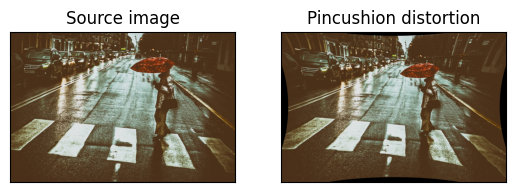
\includegraphics[width=0.7\textwidth]{my_images/41.png}
    \caption{Подушкообразное искажение}
\end{figure}
\begin{figure}[H]
    \centering 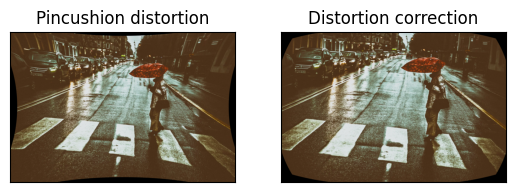
\includegraphics[width=0.7\textwidth]{my_images/42.png}
    \caption{Востановленное искажения}
\end{figure}
\begin{figure}[H]
    \centering 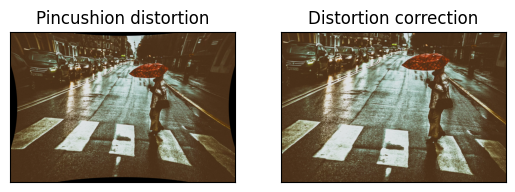
\includegraphics[width=0.7\textwidth]{my_images/43.png}
    \caption{Ещё одно востановление искажения}
\end{figure}
\section{Склейка}
Главная мысль этого метода заключается в том, чтобы найти пересекающиеся области на двух изображениях и объединить их в системе координат одного изображения.
Его запись выглядит таким образом
$$
	\begin{cases}
		x'=a_1+a_2x+a_3y, \\
		y'=b_1+b_2x+b_3y
	\end{cases}
$$
Исщем эти коэффициенты 
$$
	\begin{bmatrix}
		a_1  \\ a_2 \\ a_3
	\end{bmatrix}
	=
	\begin{bmatrix}
		1 & x_1 & y_1
		\\ 1 & x_2 & y_2
		\\ 1 & x_3 & y_3
	\end{bmatrix}^{-1}
	\begin{bmatrix}
		x'_1  \\ x'_2 \\ x'_3
	\end{bmatrix}
$$

$$
	\begin{bmatrix}
		b_1  \\ b_2 \\ b_3
	\end{bmatrix}
	=
	\begin{bmatrix}
		1 & x_1 & y_1
		\\ 1 & x_2 & y_2
		\\ 1 & x_3 & y_3
	\end{bmatrix}^{-1}
	\begin{bmatrix}
		y'_1  \\ y'_2 \\ y'_3
	\end{bmatrix}
$$
В нашем же коде мы просто пользуемся встроенной функцией OpenCV  \texttt{cv.matchTemplate()} и соединиям нами же разделённое изображение.
\begin{figure}[H]
    \centering 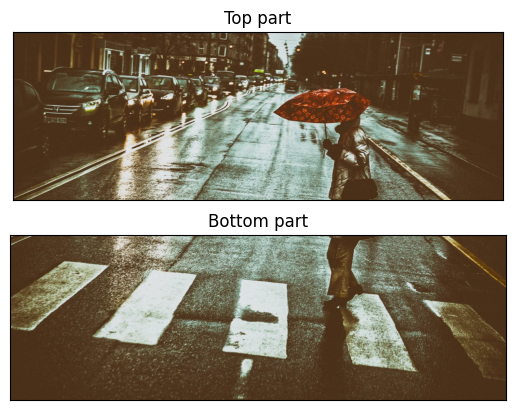
\includegraphics[width=0.7\textwidth]{my_images/44.png}
    \caption{Поделённое на части изображение}
\end{figure}
\begin{figure}[H]
    \centering 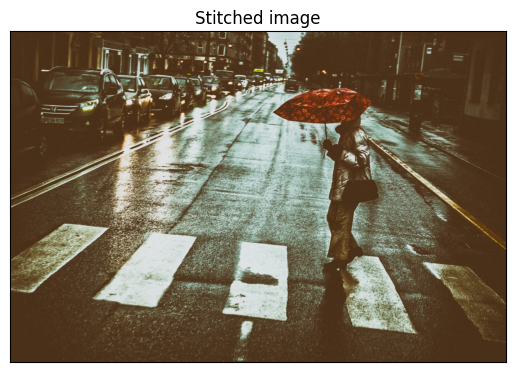
\includegraphics[width=0.7\textwidth]{my_images/45.png}
    \caption{Склейка}
\end{figure}
Также OpenCV имеет свой собственный класс, который автоматически склеивает изображения. Вот некоторые из результатов.
\begin{figure}[H]
    \centering 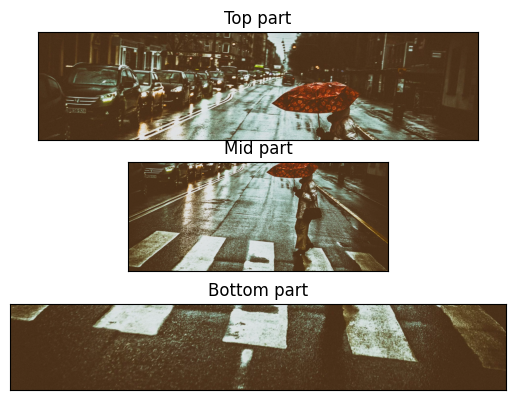
\includegraphics[width=0.7\textwidth]{my_images/46.png}
    \caption{Сложно поделённое изображение}
\end{figure}
\begin{figure}[H]
    \centering 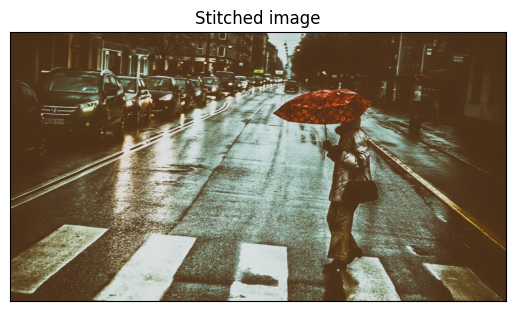
\includegraphics[width=0.7\textwidth]{my_images/47.png}
    \caption{Склейка от OpenCV}
\end{figure}
\section{Вопросы и выводы}
\begin{enumerate}
\\
\\
\item How can you rotate an image without using a rotation matrix?
\\
\\
 Вместо матрицы поворота можно последовательно применить два скоса по разным координатными осям.
 \\
\item What is the minimum number of corresponding pairs of points that must be specified on the original and distorted images to correct a perspective distortion?
\\
\\
 Четыре, но они по тройкам не должны лежать на одной прямой.
\\
\item After geometric transformation of the image, pixels with undefined intensity values may appear. What is the reason for this and how can this problem be solved?
\\
\\
Не все наши преобразования являются биективными + пиксели это дискретные объекты, поэтому могут возникать разрывы. К примеру если мы растягиваем коодринату x в два раза (т.е умножаем на 2), то логично, что в новом изображении появятся "дырки" на нечётных местах. Также такие ошибки могут возникнуть из-за ошибок округления. 
 Такую проблему можно решать с помощью интерполяции пустого пикселя за счёт окружающих его. Как можно заметить, всегда, когда мы использовали функции из openCV, которые как либо растягивали изображение, то мы указывали параметр interpolation, чтобы избежать этой проблемы.
\end{enumerate}

\section{Выводы}
В данной лаб. работе мы смоглии поработать с разными методами геометрических преобразований изображений. Как линейными, так и нет. Как оказалось достаточно много из преобразований можно получить с помощью методов линейной алгебры. 
Также мы смогли востановить изображения после несильных искажений, возникающих из-за свойств линз, что может оказаться довольно полезным в будущем. Склейка также выглядит довольно полезно.

В совокупности все эти методы могут оказаться невероятно полезными для преобразования и востановления изображений.


\end{document}
